\documentclass[english,a4paper]{article}

\usepackage[T1]{fontenc}
\usepackage[latin9]{inputenc}
\usepackage[english]{babel}
\usepackage{lmodern}
\usepackage{hyperref}
\usepackage{color}
\usepackage{url}
\usepackage{verbatim} 

\usepackage{graphicx}
\usepackage{float}
\graphicspath{{./figures/}}
\begin{document}


\title{Click-stream Data Analysis of Web Traffic}
\author{Riivo Kikas, Karl Potisepp}
\date{\today}
\maketitle

\begin{abstract}
In  this paper, we will conduct a case study of mining frequent user access patterns from web log files.
\end{abstract}





\section{Introduction} 
Understanding how users navigate and browse through web sites is important in many aspects, such as content recommendation,
personalization and targeted advertising. Even more, it helps to understand users' needs and helps and provides real world input to better organization of content and structure.

The aim of this report is to illustrate pattern mining from web logs with example of web access logs from the public web site of the Faculty of Mathematics and Computer Science of the University of Tartu\footnote{\url{http://math.ut.ee}}. Motivation for this study was to find meaningful use-cases from log files and identify possible bottlenecks in the presentation layer and provide some input for user interface redesign. 


The primary objective was to discover the most frequent sequences by analyzing the visitors' browsing sessions. The nature of pattern mining carried out was mainly exploratory, concentrating on frequent item sets and sequence mining.

Write here about sessions and data. And the overview of the process








\section{Data preparation} 
For each time an user visits a web page, a piece of information is typically stored in a web server's log file. When user navigates around a website, all such pieces of information (alternatively called requests or clicks) form a session (click-stream). We consider a session as an user's single visit to the website and associate each click with to one session.

Input data is stored in website log files, namely in Common Log Format\cite{ref_clf} format. Each log entry consists of :(i) User's IP address, (ii) Access time, (iii) Request method (\emph{GET}, \emph{POST}), etc), (iv) URL of the page accessed, (v) Prototcol (typically HTTP/1.0), (vi) Return code, (vii) Number of bytes transmitted\ref{log_sample}.

It must be mentioned, that log files contain all HTTP requests made to the web server, including requests for downloading images and style sheet documents attached to the web pages served.

\begin{figure}[h]
{\tiny
\begin{verbatim}
192.168.1.245 - - [13/Sep/2009:04:07:56 +0300] "GET /ati/struktuur/tiiger HTTP/1.0" 200 19828
192.168.1.215 - - [13/Sep/2009:04:09:30 +0300] "GET / HTTP/1.0" 200 13511
192.168.1.215 - - [13/Sep/2009:04:12:02 +0300] "GET /103369 HTTP/1.0" 200 17367
192.168.1.215 - - [13/Sep/2009:04:14:40 +0300] "GET /varia/itinfo HTTP/1.0" 200 19411
\end{verbatim}
}
\label{log_sample}
\caption{Example of log file}
\end{figure}

Two important tasks must be performed before clickstream data from \emph{CLF} files can be used for analyzing: data cleaning and session identification.







\subsection{Data cleaning}
Since log files contain all requests made to the server, we need to extract only relevant requests and eliminate others. When filtering requests from log files, following rules were applied:

\begin{itemize}
\item Only requests to the public site are considered. Requests to personal homepages (pages starting with ~) are discarded. Also, all static content files that were used by web pages were removed, such as image files, JavaScript and CSS documents. \\ The server also had had special error page url, that the user was redirected to when they tried to access a non-existant resource. We eliminated this kind of access requests, as these are not initially made by users. It must be noted that the request for the original page that caused the server to redirect the user remains in the log file.
  
\item All other HTTP request types besides POST and GET were ignored. We noticed that there were regular OPTIONS request, that most probably were made by some automated monitoring tool. 
  
\item We composed a blacklist of of IP addresses, whose requests were all ignored. An IP address was added to blacklist, if there was a request made from the IP address to access \emph{robots.txt} file. Namely, we believe that only automated indexers request robot.txt and therefore we can ignore all subsequent requests from those IP-s, since we are only interested in how a human user perceives the web site. 
\end{itemize}


In addition to that, we modified requested URLs by removing query string attributes(the part of the URL that starts with ?). We assumed that typically URLs identify a distinct page and query-string some operation or action on it. This helped us to reduce number of different URLs while preserving meaningful information about the usage patterns.

After performing all the procedures described above, the log files now contain only information about the HTTP requests originating from intentional clicks made by the users on pages. These requests can be grouped into users' click-streams.











\subsection{Session identification}
The next step was to group user requests made during one visit into sessions. A user session is defined as a sequence of temporally compact accesses by a user \cite{on_mining_logs}.

Generally, this can be done by providing a cookie to each user with some generated unique identification number and then logging each request and the cookie ID simultaneously. However since log files in CLF do not store an explicit session ID, and since we could not modify the existing software stack, we had to use the data that was already given.  

As a solution, we used a timeout based method to group requests into sessions. We consider a sequence of requests from the same IP address ordered by time to be in
same session, if the time between consecutive requests (clicks) is not more
than $t = 30$ minutes. If time between requests exceeds $t$, we
consider these requests to be part of a new session. While this method is
probably not the best, we consider it sufficient as it mimics the way session
timeouts are measured on many web sites. We also consider it reasonable to
assume that if an user has not interacted with the server for more than $t$
minutes, any new interaction from an user from the same IP address can be
thought of as a new use case scenario.










\subsection{Statistics about the logs} 
The log files contained info about requests made to the server from August to December 2009, with October data missing. In total, log files contained 
$544237$ requests, of which $122822$ remained after data cleaning. These requests were grouped to $35952$ sessions. Average session length was $??$. Distribution of user session length can be see on figure \ref{session_len}. Requests involved $2059$ distinct URLs. 

\begin{figure}[H]
  \centering
      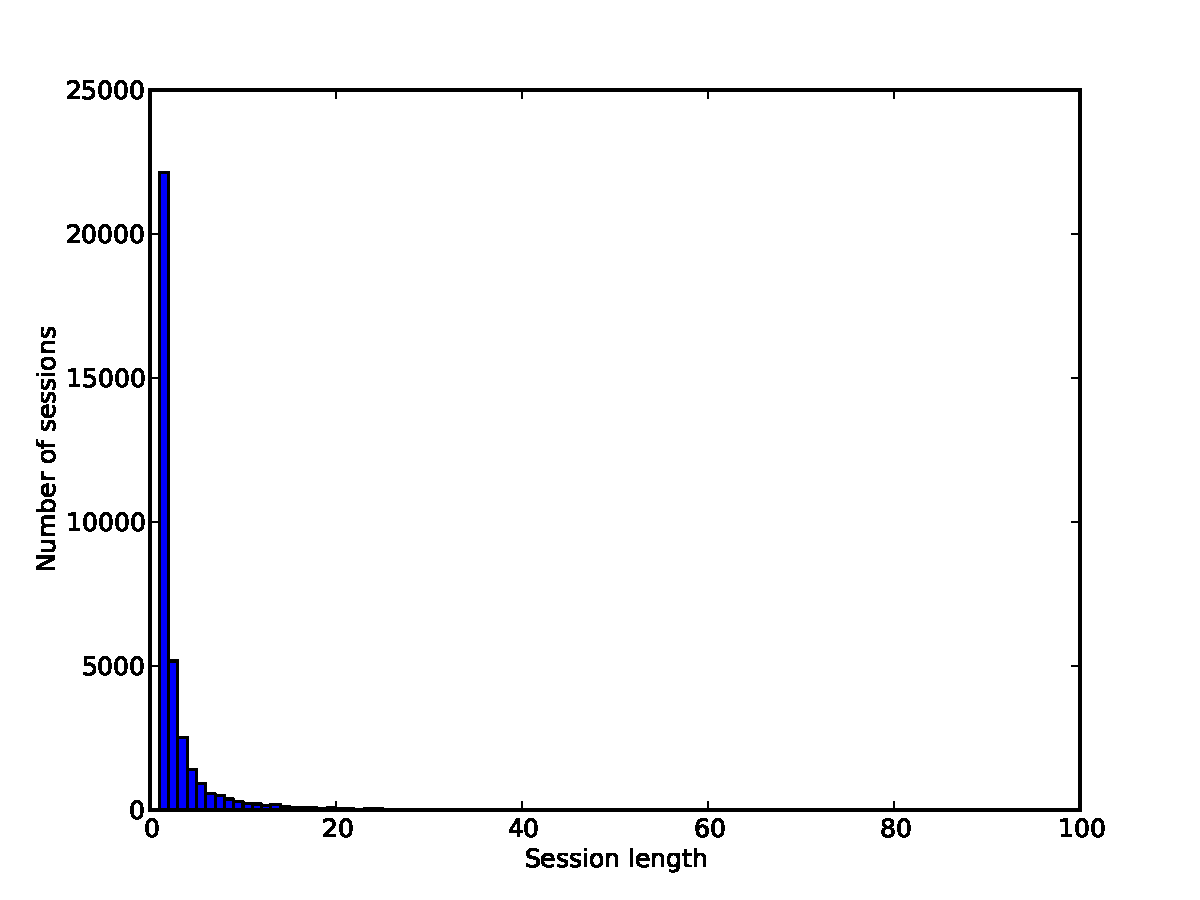
\includegraphics[width=0.9\textwidth]{session_len}
  \caption{Session length histogram}
  \label{session_len}
\end{figure}

















\section{Frequent item sets} 
From the perspective of web site design and browsing sessions, the most important question is whether or not there are groups of pages users tend to visit together. The presence of such kinds of groups can give a web designer valuable insight into how people use the web site. For example, content split on separate pages but still often viewed together can be merged to achieve a smoother browsing experience.

We approached the task of identifying such groups by thinking of every page as a unique \emph{item}, which then form sets, each containing pages visited during one browsing session. To find pages that are frequently visited together, we searched among these sets for subsets of pages that frequently appear together. The problem now was deciding when a subset of pages is frequent. We solved this by using a set mining \cite{frequent_item_set_mining} tool called \emph{support}.

Support is a number that shows how frequently a subset appears in all item sets. Using this concept, it is trivial to eliminate subsets that are not common. The only problem is that there is no magic bullet solution to choosing the 'right' support threshhold. A value too high does not provide insight into more specific subsets, a value too low results in too much non-frequent garbage.

\begin{figure}[H]
  \centering
      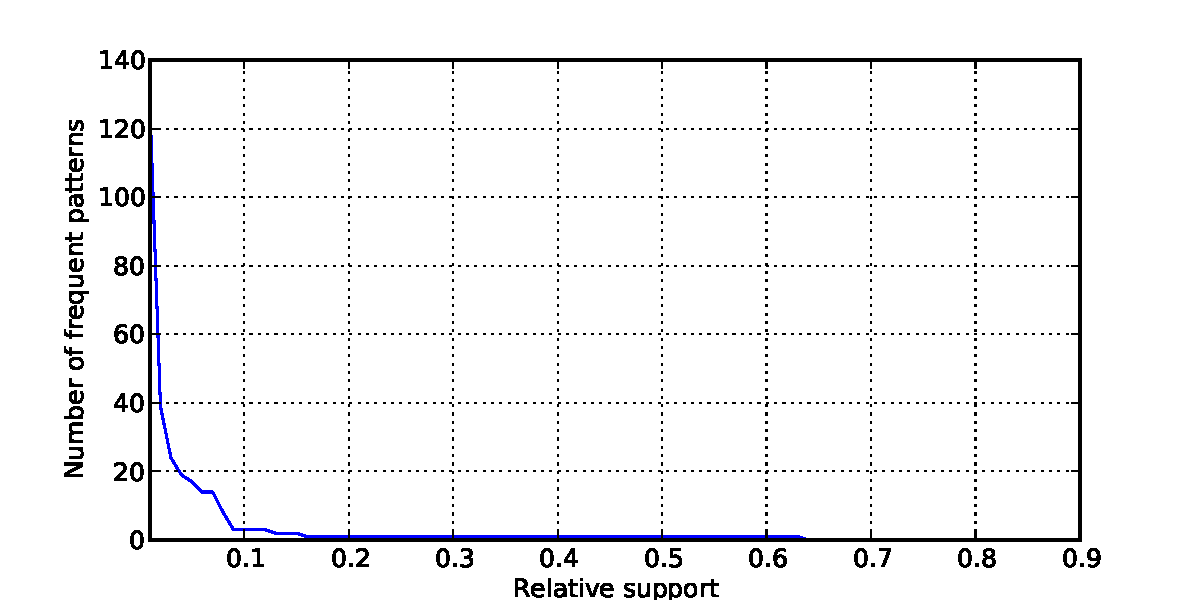
\includegraphics[width=0.9\textwidth]{apriori_closed_itemset_count}
  \caption{How rule support changes number of frequent itemsets}
\end{figure}


However even if we manage to choose an optimal value for the support threshhold, after filtering out all the infrequent subsets, some redundancy remains in the results. It is easy to see that if a set of 5 pages appears frequently throughout the sessions, all 4 page subsets of that set appear at least as frequently. To eliminate this kind of noise, we used another concept: \emph{closed item sets}. An item set is closed if all its proper supersets have smaller support. By searching for only closed item sets, we eliminate uninteresting subsets of already present results and leave only those which provide useful information.

We used the following algorithm to find frequent closed itemsets.

In addition to the difficulties in choosing an ideal support threshhold, there are other problems with this approach to detecting pages frequently requested during one session. While we can easily find groups of pages that are probably viewed together, much more insight could be gained if we knew the order in which the pages were navigated. Knowing this we would also gain information on how the users find what they need on the site. Similarly, if an user visits a page several times during one session, this fact is not known to us. \emph{Frequent sequential item sets} solve these problems at least partially.







\section{Frequent sequential patterns}
Simply by listing all frequent item sets we won't see much how user actually use website. This is because of two reasons. First, frequent item sets do not capture of the order of pages visited. Secondly, information about multiple page visits is lost constructing item sets. 

The solution for this problem can be solved by mining frequent sequential item sets. Sequential pattern mining is about mining frequent event sequences from databases i.e. we are mining sequences of clicks that frequently are followed by each other. Frequent sequences can be used to see how user actually tend to navigate and reach some desired resource.

To mine frequent patterns from our dataset, we used  an \emph{a priori}-based frequent item sequence miner that uses a trie to store the candidates\cite{seq_apriori}.

\begin{figure}[H]
  \centering
      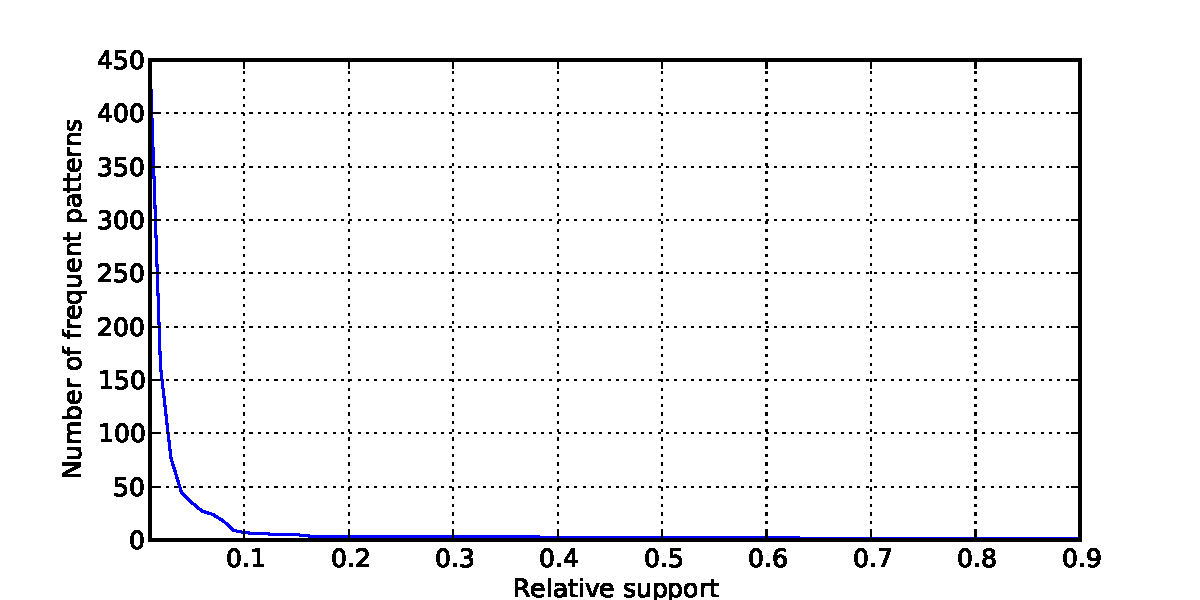
\includegraphics[width=0.9\textwidth]{sequential_itemset_count}
  \caption{Number of frequent sequential patterns depending on relative support}
\end{figure}


\subsection{Page access times}
As for every click the timestamp is available when the click was executed, we can find how much time user actually spend on a web page by calculating time interval between two clicks. For every page, we can calculate average time user spend on this page. But this is more effective, if we apply this method to previously found sequential rules. Namely, for every frequent sequence found, we look find all session that contain this sequence and calculate median time for every page in the sequence that users spend on that page.  We choose median time as we consider this more appropriate by experimental evaluation.

This methods allows us to determine the pages that are visited only because of navigation and not for content. For usability reasons, such pages should be removed to reduce user clicks.





\section{Maximal reference sequences}
Path traversal pattern mining has been studied extensively to find better alternatives to regular frequent sequence mining in web mining context. A solution has been provided \cite{path_patterns} that provides regular sequential patterns, but reduces the patterns only to \emph{forward reference sequences}, that is patterns that only contain forward navigations. Authors of \cite{path_patterns} say that forward reference illustrate what people are looking for e.g. destination pages and eliminate back references from sessions.

When applied this algorithm to our dataset, we found almost same rules as with the regular sequential pattern mining technique. The differences was only number of patterns found, namely by eliminating back references and repeating pages, we find less patterns. When  number of patterns is bigger, this methods helps to bring better overview of frequent user traversal path and target pages than previously used.

\section{Changes in patterns through time} 
Pattern mining can bring insight into how patterns changes in time. When mining school website data, one can hypothesize how users' interest changes in time. We can presume, that August is the pre-semester period and students might be looking for information about new professors, timetables, good seminars provided upcoming semester. When the semester starts in September, it can be assumed that these kinds of aims become outdated and new behavioral patterns arise.

We split up the data set into two datasets: August and  Sepetember and compared sequential rules found for both datasets with same relative support, s=$0.04\%$









\section{Restricting patterns by user specified pages}

In our dataset, number of different pages visited is relatively big compared to total number of sessions and average session length and as it can be seen support based rule mining might not find all interesting rules, without lowering support to very low. One idea how to overcome this problem and find easily more appropriate and significant frequent itemsets is following: Identify pages that you are interested in and find all sessions that contain these pages. Now run frequent pattern mining algorithms on the filtered session collection. The output should contain more relevant patterns with higher support and provides a simple way to analyze use cases separately and more thorough.

We conducted the experiment and selected session that contain page \emph{inimesed/Instituudid}. The results did not reveal anything interesting, but it helped us reveal still more patterns about the page. For example, a   frequent pattern with $40\%$ support among filtered sessions was discovered that showed how in some cases users to refresh on the front page before arriving on page \emph{inimesed/Instituudid}.

\section{Summary}
We have shown practical example how web analytics can be taken beyond google analytics and webalizer
More work could be done by reasearching into oulier detection and signifacne detection










\bibliographystyle{alpha}
\bibliography{bibliography}
\end{document}
